\subsection{Medidas de Centralidade e Variabilidade} 

\subsubsection{Centralidade}

Média - soma dos valores dos dados de um conjunto dividido pelo número de dados (elementos) constante nesse conjunto.

	\begin{figure}[h!]
		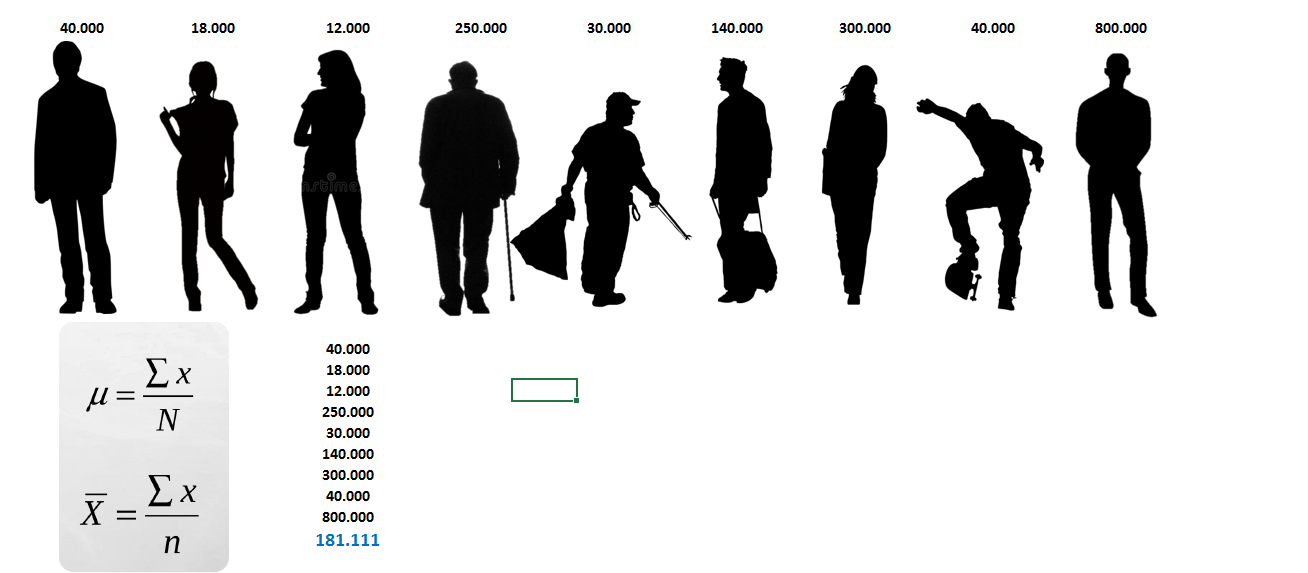
\includegraphics[scale=0.50]{cap2/MedidasCentralidadeVariabilidade/Media.png}
	\end{figure}

Moda - É o valor mais frequente num conjunto de dados.

	\begin{figure}[h!]
	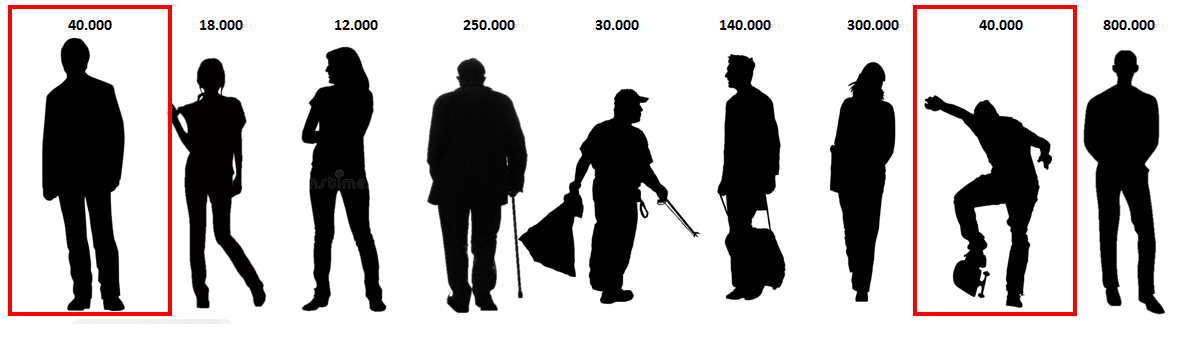
\includegraphics[scale=0.50]{cap2/MedidasCentralidadeVariabilidade/Moda.png}
	\end{figure}

\newpage

Mediana - É o valor que medeia os valores presentes num conjunto ordenado numericamente.

	\begin{figure}[h!]
	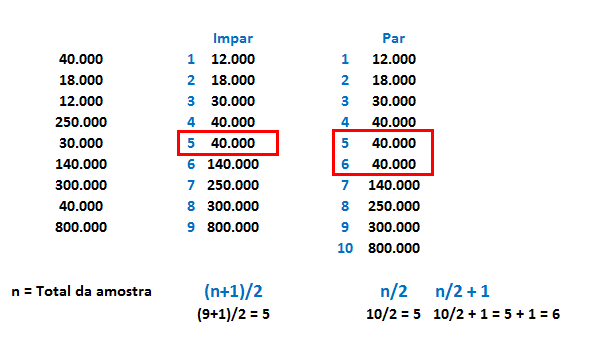
\includegraphics[scale=0.50]{cap2/MedidasCentralidadeVariabilidade/Mediana.png}
	\end{figure}

Desvio Padrão - Indica o grau de variação de um conjunto de elementos.

Como Calcular:
 
	\begin{figure}[h!]
	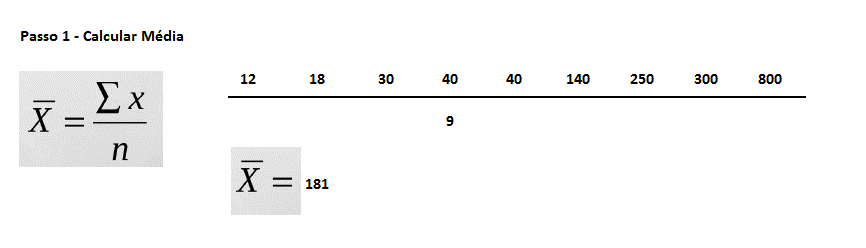
\includegraphics[scale=0.50]{cap2/MedidasCentralidadeVariabilidade/DesvioPadrao1.png}
	\end{figure}

	\begin{figure}[h!]
    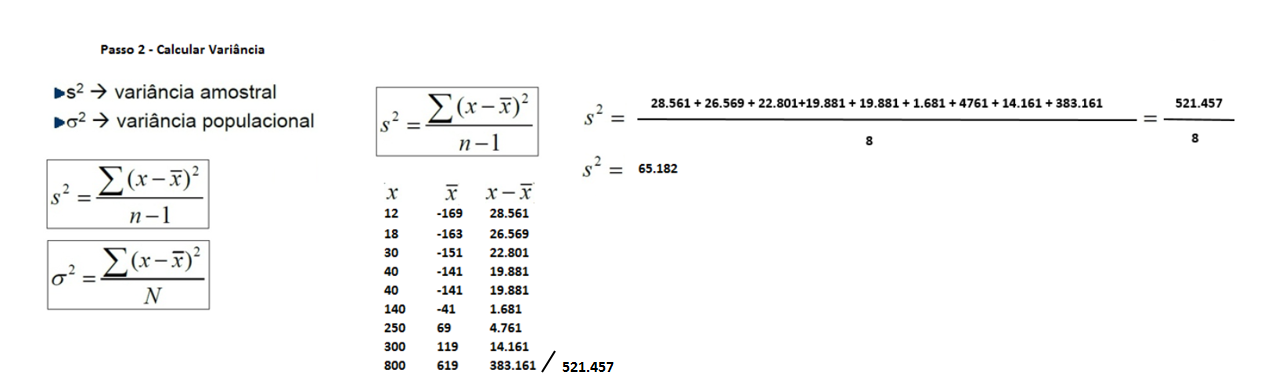
\includegraphics[scale=0.50]{cap2/MedidasCentralidadeVariabilidade/DesvioPadrao2.png}
	\end{figure}

	\begin{figure}[h!]
    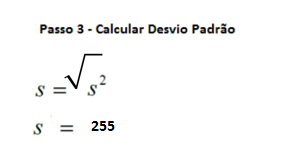
\includegraphics[scale=0.50]{cap2/MedidasCentralidadeVariabilidade/DesvioPadrao3.png}
  	\end{figure}
  
\newpage
Amplitude - Em estatística, a amplitude representa a diferença entre o maior e o menor valor de um conjunto de dados.

	\begin{figure}[h!]
	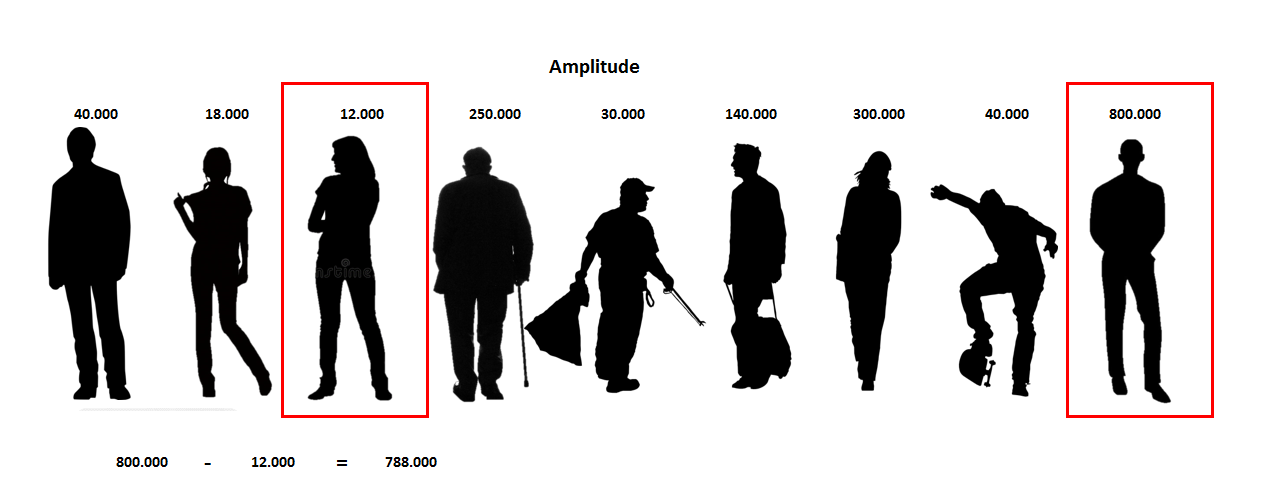
\includegraphics[scale=0.50]{cap2/MedidasCentralidadeVariabilidade/Amplitude.png}
	\end{figure}


Quartis (Q1, Q2 e Q3): São valores dados a partir do conjunto de observações ordenado em ordem crescente, que dividem a distribuição em quatro partes iguais. 
O primeiro quartil, Q1, é o número que deixa 25\%\  das observações abaixo e 75\%\ acima, enquanto que o terceiro quartil, Q3, deixa 75\%\ das observações abaixo e 25\%\ acima. Já Q2 é a mediana, deixa 50\%\ das observações abaixo e 50\%\ das observações acima. Mais informações sobre quartil  \href{http://www.portalaction.com.br/estatistica-basica/23-quartis}{Quartis}

	\begin{figure}[h!]
	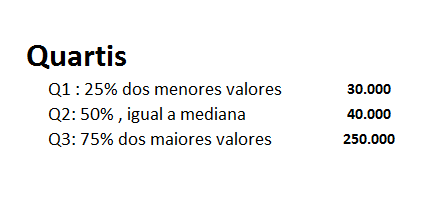
\includegraphics[scale=0.50]{cap2/MedidasCentralidadeVariabilidade/Quartil.png}
	\end{figure}

	\begin{figure}[h!]	
	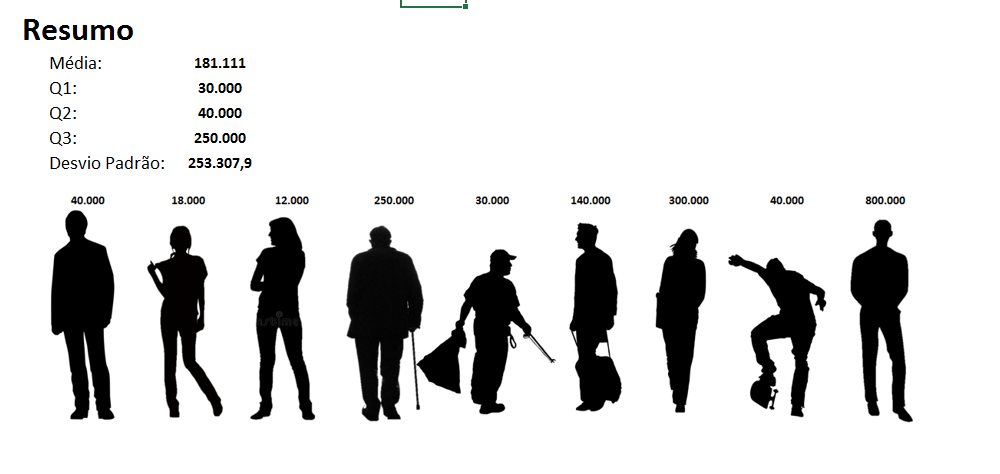
\includegraphics[scale=0.35]{cap2/MedidasCentralidadeVariabilidade/Resumo.png}
	\end{figure}

 
\newpage
  
\subsubsection{Centralidade - R}

Para realizarmos os testes vamos criar a variável jogadores, com os mesmos salários da 
imagens.
\\\\Variável
\\jogadores = c(40000, 18000, 12000, 250000, 30000, 140000, 300000, 40000, 800000)\\
\\Calcula a média
\\mean(jogadores)
\\\\Calcula a mediana
\\median(jogadores)
\\\\Calcula os Quartis 
\\quartis = quantile(jogadores)
\\\\ver os quartis 
\\quartis
\\\\ver o terceiro quartil 
\\quartis[4]
\\\\Calcula o Desvio Padrão
\\sd(jogadores)
\\\\Mostra o resultado da variável 
\\summary(jogadores)
\\summary(jogadores)

\newpage
Resultados:

	\begin{figure}[h!]	
	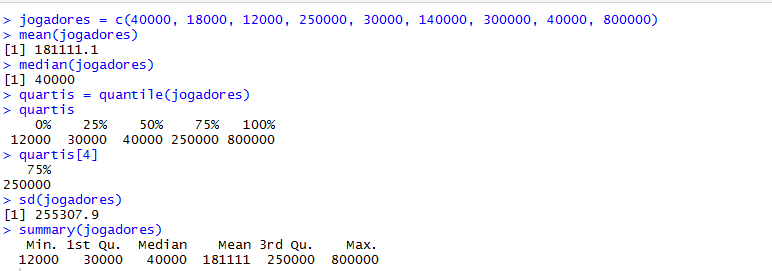
\includegraphics[scale=0.90]{cap2/MedidasCentralidadeVariabilidade/MedidasCentralidadeVariabilidadeR.png}
	\end{figure}

	\begin{figure}[h!]	
	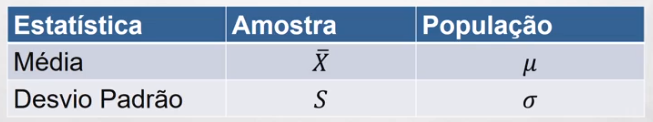
\includegraphics[scale=0.90]{cap2/MedidasCentralidadeVariabilidade/AmostraEPopulacao.png}
	\end{figure}

